\documentclass{article}
\usepackage{tikz}
\usetikzlibrary{shapes,arrows}
\usepackage{caption}
\begin{document}
	\begin{titlepage}
    	\title{Master controller definition}
    	\author{Michael King, 200402171}
    	\maketitle
    	\thispagestyle{empty}
	\end{titlepage}
    \begin{abstract}
        The purpose of this document is to define the requirements and provide a
         simple work plan for the Master controller main module. This document 
         will include a simple block diagram and a flowchart for expected 
         operations
         \newpage
	\end{abstract}
    \section{Introduction}
        The Master Controller will be the most complex single part of the entire
         project, the purpose of the master controller is to act as a gateway
         between the wired and wireless networks, display errors, provide a
         power supply for wired devices, and provide a simple menu for viewing 
         devices on the network.
     
     \section{System definition}
     The block diagram shown in figure~\ref{fig:simpleblock} is meant to
     encompass the components contained within the enclosure of the Master
     controller main unit. Some simplifications have been made, the A/C
     power supply will be connected to everything. And likely separate from
     the PCB that most of the rest of the components will be located on.
     \begin{figure}[htp]
	     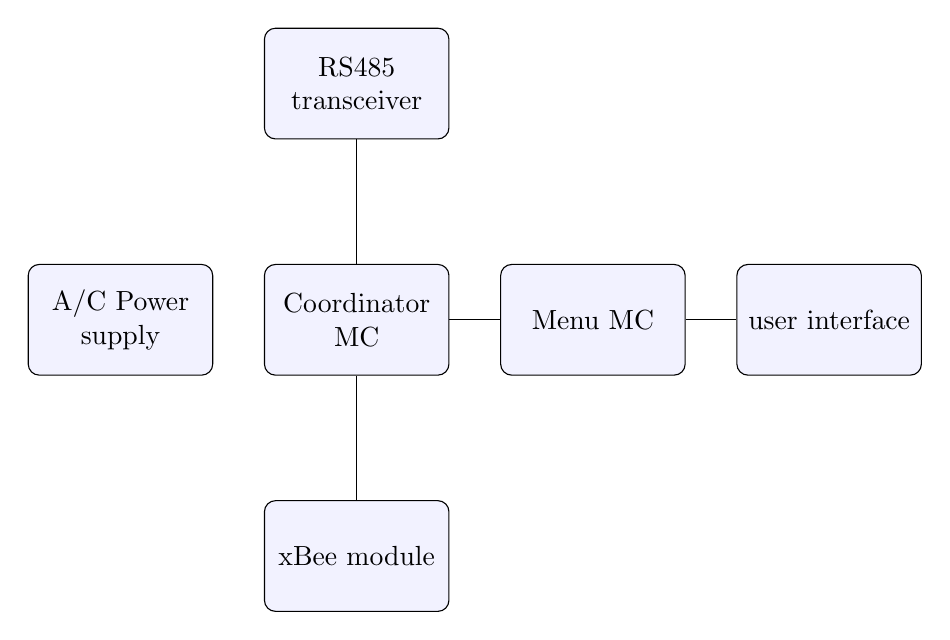
\begin{tikzpicture}[auto, node distance=3cm,>=latex']
    	 	% Define block styles
    	 	\tikzstyle{block} = [rectangle, draw, fill=blue!5, text width=6em, text centered, rounded corners, minimum height=4em]
    	 	\tikzstyle{line} = [draw, -]
    	 	
    	 	% Nodes
    	 	\node [block] (coordinator mc) {Coordinator MC};
    	 	\node [block, right of=coordinator mc] (menu mc) {Menu MC};
    	 	\node [block, below of=coordinator mc] (xBee) {xBee module};
    	 	\node [block, right of=menu mc] (user interface) {user interface};
    	 	\node [block, above of=coordinator mc] (RS485) {RS485 transceiver};
     		\node [block, left of=coordinator mc] (Power Supply) {A/C Power supply};
     	
    	 	% Connecting lines
     		\path [line] (coordinator mc) -- (menu mc);
     		\path [line] (menu mc) -- (user interface);
     		\path [line] (coordinator mc) -- (xBee);
     		\path [line] (coordinator mc) -- (RS485);
     	\end{tikzpicture}
     	\caption{block diagram representing subsystems within the enclosure of the Master Controller}
     	\label{fig:simpleblock}
     \end{figure}
     \newline 
     A decision was made to place separate microcontrollers within the Master Controller to allow
     the coordinator micro to be focuses entirely on coordinating messaging between the wired 
     and wireless networks, while the menu micro only needs to display messages from the coordinator
     and keep track of a device list.
     \newpage
     \section{operations}
     	see figure~\ref{fig:simpleflowRS485RX} for a simplified flowchart of the operation of the Master
     	 Controller main unit.
     	\subsection{coordinator}
     		The coordinator's primary task is to perform coordination between the wired and wireless
     		 networks, but it will also filter out system messages to send to the menu controller,
     		 and assign devices on the wired network. And potentially provide collision detection 
     		 for its connected control modules on the wired network.
     		 As such, it needs to be capable of keeping a large amount of device a names in memory for 
     		 quick reference when messages arrive. And have a reasonable buffer for messages.
             We will target having enough memory for at least 1024 wireless devices.
             most likely, this will be a 3.3v device so that it can use the same 
             voltage regulator as the xbee module
     	\subsection{menu}
     		The menu micro spends most of its time listening for system messages from the coordinator 
     		these may be error messages, or other general status (i.e. new device joins network). The 
     		menu micro is responsible for managing the user interface as well.
     	\subsection{user interface}
     		The user interface consists of two parts: some type of display managed by the menu micro, 
     		And some type of user input to navigate through a log of system messages, and a simple 
     		device map.
     	\subsection{power supply}
     		The primary wired A/C power supply may be located within the master controller enclosure, 
     		the purpose of this is to provide power to all wired modules (with the possible exception 
     		of the lap counter display.) This will most likely be a 12v power supply.
     	\subsection{RS 485 Transceiver and xBee module}
     		These serve as the link between the coordinator and the rest of both networks. The xBee 
     		module is constrained to 3.3V. xBee modules provide an expected range
             of nearly 1km, with communication rates in the dozens of kbps.\ while
             RS485 can be expected to have a range of at least 1km, with a data 
             rate in the 100's of kpbs. Both of which should exceed our 
             requirements.
     \begin{figure}[htp]
     	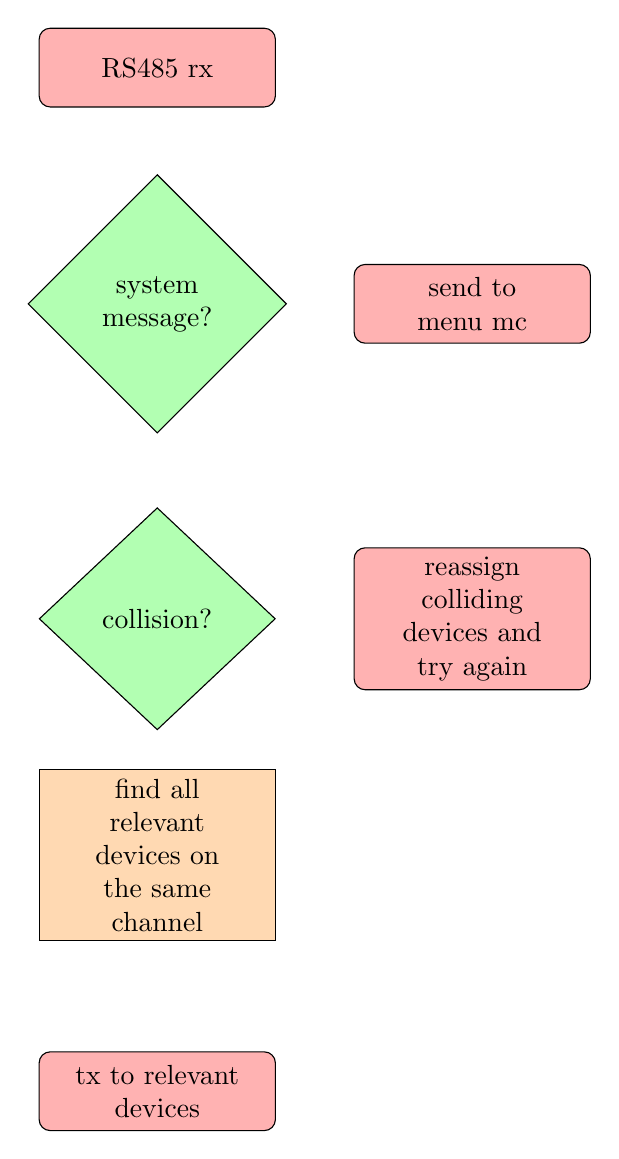
\begin{tikzpicture}[auto, node distance=3cm,>=latex']
     		%define block styles
     		\tikzset{
     			startstop/.style={rectangle, rounded corners, minimum width=3cm, text width=6em, minimum height=1cm, text centered, draw=black, fill=red!30},
     			process/.style={rectangle, minimum width=3cm, minimum height=1cm, text width=6em, text centered, draw=black, fill=orange!30},
     			decision/.style={diamond, minimum width=3cm, minimum height=1cm, text width=6em, text centered, draw=black, fill=green!30},
     			arrow/.style={thick,->,>=stealth},}
     		%define nodes
     		\node[startstop](rx){RS485 rx};
     		\node[decision, below of=rx](errcheck){system message?};
     		\node[startstop, right of=errcheck, xshift=1cm](display){send to menu mc};
     		\node[decision, below of=errcheck, yshift=-1cm](collcheck){collision?};
     		\node[startstop, right of=collcheck, xshift=1cm](reassign){reassign colliding devices 
            and try again};
            \node[process, below of=collcheck](channel){find all relevant devices 
            on the same channel};
            \node[startstop, below of=channel](xBee tx){tx to relevant devices};
     	\end{tikzpicture}
     	\caption{RS485 RX flowchart}\label{fig:simpleflowRS485RX}
     \end{figure}
\end{document}